\section{Product Overview}

The Frevia project is a comprehensive freelancing platform that enables clients, freelancers, and administrators to build trusted professional relationships and efficiently manage the entire project lifecycle. Designed to connect businesses with skilled talent worldwide, Frevia provides intelligent job matching, structured contract workflows, and secure payment solutions to facilitate successful collaborations.

Through AI-powered recommendations, real-time communication, and advanced moderation mechanisms, the platform helps users discover suitable opportunities, deliver high-quality work, and maintain transparent interactions.

Frevia serves three primary stakeholder groups: clients seeking specialized expertise, freelancers showcasing their skills and services, and administrators responsible for maintaining platform integrity and operational efficiency. The platform offers an intuitive user experience, dynamic communication channels, and comprehensive management capabilities to support collaboration, professional growth, and secure transactions.

Key features of Frevia include:

\begin{itemize}
  \item \textbf{Smart Job Matching and AI Recommendations:} The platform analyzes freelancer skills, experience, and preferences to recommend relevant job opportunities. AI-powered profile scoring provides quality assessments, while job alerts and saved searches help users stay informed about new opportunities.

  \item \textbf{End-to-End Contract and Milestone Management:} Clients and freelancers can negotiate project terms, define milestones and tasks, monitor progress, and securely manage payments. Integrated contract signing, activity logs, and file-sharing capabilities ensure transparency throughout the project lifecycle.

  \item \textbf{Community and Forum Engagement:} Frevia includes a community forum where users can discuss industry topics, exchange knowledge, and seek professional advice. Features such as categories, posts, comments, reactions, and reporting mechanisms encourage active participation and self-moderation.

  \item \textbf{Identity Verification and Content Moderation:} Freelancers can verify their identities through document submission, while administrators utilize moderation tools, banned keyword management, and AI-assisted violation detection to maintain a secure and trustworthy environment.

  \item \textbf{Wallet, Payments, and Gas Fee Subsidies:} Users can manage account balances, withdraw earnings, and review transaction histories. The platform also supports gas fee subsidy mechanisms for blockchain-based transactions, improving payment accessibility and reducing operational costs.

  \item \textbf{Administrative Management Tools:} Administrators have access to comprehensive management functionalities, including user administration, role and permission control, system configuration, advertisement management, activity monitoring, and dispute resolution, ensuring fair and reliable platform operations.
\end{itemize}

\begin{figure}[htbp]
    \centering
    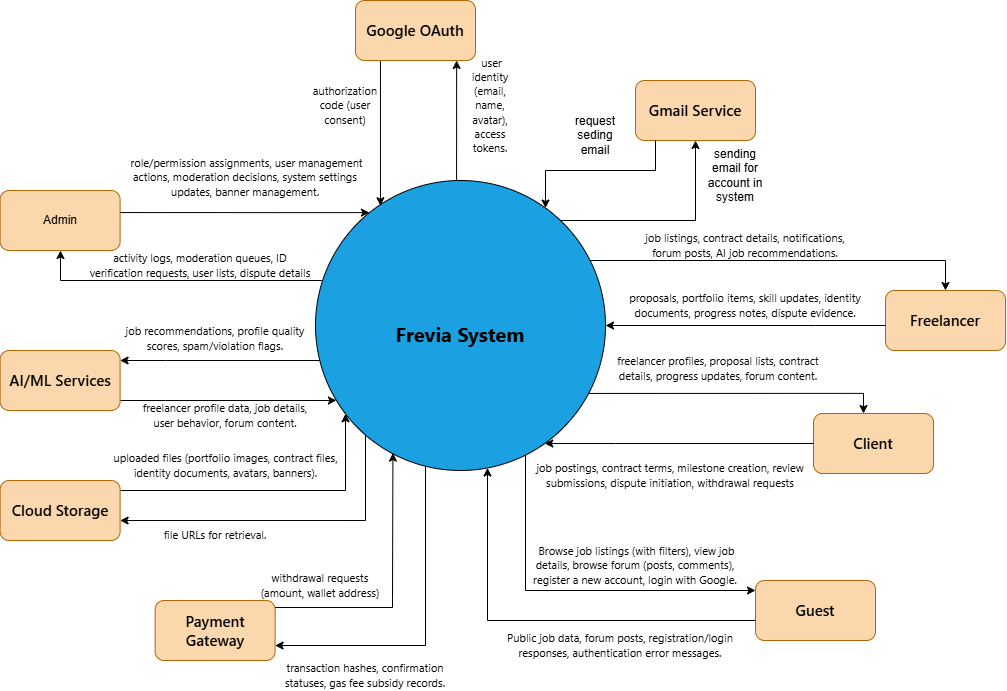
\includegraphics[width=0.9\linewidth]{image/context_diagram/context-diagram.drawio.png}
    \caption{Context diagram}
    \label{fig:context-diagram}
\end{figure}